\documentclass[utf8]{ctexart}
\usepackage{tabularx,makecell,multirow,diagbox}
\usepackage{graphicx,bm,amsmath,tikz,algorithm,algorithmicx,listings}
\usepackage{float,forest}
\usetikzlibrary{trees}
\usetikzlibrary{automata, positioning, arrows,shapes.geometric}
\usepackage[bookmarks=true,colorlinks,linkcolor=black]{hyperref} % 导入制作目录链接

\title{编译原理复习总结}

\begin{document}

\maketitle
\tableofcontents
\thispagestyle{empty} % 首页不设置页码
\newpage

% Define block styles
\tikzstyle{decision} = [diamond, draw, fill=blue!20, 
    text width=4.5em, text badly centered, node distance=3cm, inner sep=0pt]
\tikzstyle{block} = [rectangle, draw, fill=blue!20, 
    text width=5em, text centered, rounded corners, minimum height=4em]
\tikzstyle{line} = [draw, -latex']
\tikzstyle{cloud} = [draw, ellipse,fill=red!20, node distance=3cm,
    minimum height=2em]

\setcounter{page}{1} % 从内容开始重新生成页码

\section{从源代码到目标代码的步骤}
\begin{enumerate}
    \item 源代码
    \item 词法分析程序:逐个读入源程序字符并按照 构词规则 切分成一系列单词(token).单词是语言中具有独立意义的最小单位,包括保留字、标识符、运算符、标点符号和常量等
    \item 语法分析程序(描述各语法成分的形式或结构):语法分析以词法分析程序输出的单词序列(或流)为输入,分析源程序的语法结构,判断它是否为相应程序设计语言的合法程序,并可以确定单词流中违反源语言结构规则的错误
    \item 语义分析程序(各语法成分的含义或功能)
    \begin{itemize}
        \item 语法特征描述各语法成分的形式或结构
        \item 语义特征描述各语法成分的含义与功能
        \item 语义分析是在语法分析程序确定出语法短语后,审查有无语义错误,并为代码生成阶段搜集符号属性信息
        \item 语义属性包括变量的声明、计算表达式的值、语义分析包括类型检查等
    \end{itemize}
    \item 中间代码生成:为了处理方便和便于代码优化,通常在语义分析后并不直接产生目标代码,而是生成介于源代码和目标代码二者之间的中间代码
    \begin{itemize}
        \item 常数表:存放在编译过程中用到的常量和字符串,快速插入和查找操作在常数表中十分重要
        \item 符号表:存储函数、变量、常量以及数据类型等标识符相关的信息
        \begin{itemize}
            \item 在词法分析、语法分析和语义分析的过程中收集有关标识符的属性,并存于符号表中
            \item 作为进行语法和语义的合法性检查的依据
            \item 作为目标代码生成阶段地址分配的依据
        \end{itemize}
    \end{itemize}
    \item 代码优化程序:对产生的中间代码进行等价变换或改造
    \item 目标代码生成
    \item 编译阶段的组合
    \begin{itemize}
        \item 前端:与目标机无关的部分,包括分析部分(词法、语法、语义分析)、中间代码生成与优化以及这部分的符号表管理错误处理
        \item 后端:与目标机有关部分包括目标代码生成、与目标机有关的优化以及这部分的符号表管理和错误处理工作
    \end{itemize}

    \item 交叉编译:在计算机M1(宿主机)上编译出计算机M2(目标机)的目标程序
\end{enumerate}


\section{词法分析}
\noindent 词法分析器的任务:
\begin{itemize}
    \item 从源代码中读取输入字符,按照构词规则切分成一系列单词,提交给语法分析使用。
    \item 识别出源程序中的单词
    \item 删除无用的空白字符及注释
    \item 检测出输入的源程序中不能形成源语言任何单词的错误字符串
\end{itemize}

\subsection{正规表达式(单词的描述工具)}
\noindent 基本概念
\begin{itemize}
    \item 字母表(符号表、符号集):由若干元素(符号、字母)组成的有限非空集合称为字母表
    \item 符号串:由字母表中的符号组成的任何有穷序列称为符号串
    \item 符号串的长度:如果某个符号串$x$中有$m$个符号,称其长度为$m$,表示为$|x|=m$
    \item 空符号串$\epsilon$,不包含任何符号的符号串,其长度为0,即$|\epsilon|=0$
    \item 符号串的连接:设$x$和$y$是符号串,他们的连接$xy$是把$y$的符号写在$x$的符号之后得到的符号串。$\epsilon x=x\epsilon=x$
    \item 符号串的方幂:符号串自身连接$n$次得到的符号串$x^n$定义为$xx \dots xx$;$x^0 = \epsilon$
    \item 符号串集合(或语言):若集合$A$中所有元素都是某字母表$\sum$上的符号串,则称$A$为字母表$\sum$上的符号串集合
    \item 符号串集合的操作
    \begin{itemize}
        \item 并(和):与集合的并运算一致
        \item 连接:笛卡尔积
        \item 闭包:集合的闭包
        \item 正闭包:不包含$\epsilon$的闭包
    \end{itemize}
\end{itemize}

\noindent \textbf{正规表达式}

定义:是用特定的运算符及运算对象按照规则构造的表达式,每个正规表达式匹配一个字符串的集合(称为正规集);设有字母表为$\sum$(运算对象),
辅助字母表${\sum}^{'}=\{\Phi,\epsilon,|,.,*,()\}$(运算符优先级为先“ ( )”,“ * ”,再“ . ”最后“ | ” ,它们满足左结合律),正规表达式和它所表示的正规集(字符串的集合)的递归定义如下:
\begin{enumerate}
    \item $\epsilon$和$\Phi$是$\sum$上的正规式,他们所表示的正规集分别为\{$\epsilon$\},\{\}
    \item 若$a \in \sum$,则$a$是$\sum$上的正规式,它所表示的正规集为$\{a\}$
    \item 若r和s是Σ上的正规式,他们所表示的正规集分别为L(r)和L(s),则
    \begin{itemize}
        \item $r|s$是正规式,表示的正规集为 $L(r|s)=L(r) \cup L(s)$
        \item $rs$是正规式,表示的正规集为$L(rs)=L(r)L(s)$
        \item $r^*$是正规式,表示的正规集为$(L(r))^*$
        \item $(r)$是正规式,表示的正规集为$L(r)$
    \end{itemize}
    \item 有限次使用上述步骤3而定义的表达式是Σ上的正规式,由这些正规式所表示的符号串集合是Σ上的正规集 
\end{enumerate}

作用:描述语言词法规则的形式化工具。给定一个正规式,它唯一确定一个正规集;给定一个正规集,则可由多个不同的正规式表示。
若两个正规式描述同一正规集,则称两个正规表达式等价(判断两个正则表达式是否等价等同于判断两个正则表达式的最小化DFA是否相等)


正规表达式的扩展
\begin{itemize}
    \item $r^+$:$r$被重复1次或更多次
    \item .:表示可以匹配除换行符之外的任意单个字符
    \item {``''}:引号中的字符表示文本字符串本身
    \item 字符范围$[]$
    \item 为正规表达式命名
    \item 可选的子表达式:?
\end{itemize}

\subsection{有穷自动机(DFA, Deterministic Finite Automata)}
\subsubsection{确定性有穷自动机}
定义:由下述五元式$M=(S,\sum ,T,S_0,A)$称为一个确定的有限自动机
\begin{enumerate}
    \item 有限个符号组成的字母表,记做$\sum$
    \item 有限个状态的集合,记作S
    \item 转化函数T:$S \times \sum  \rightarrow S$即$T(s,c)=s^{'}$,
    其中$s\in S, s^{'} \in S,c \in \sum$,表示若当前状态为s,且当前识别的输入符号为c,识别c后进入的下一个状态为$s^{'}$
    \item 初始状态$s_0 \in S$,指示识别符号串的起始位置
    \item 若干个识别符号串的接受状态(终止状态)的集合$A\subseteq S$
\end{enumerate}

\noindent \textbf{状态转换图}
\begin{enumerate}
    \item m个状态就有m个节点,用箭头指示初始状态,用双圆圈表示终止状态
    \item 若 T(s,a)=s’ ,则从状态结点s到状态结点s’画标记为a的矢线
    \item 隐含的错误状态没有绘制,状态可以使用任何标识系统来标识,转化可以使用字符集合的名字标出
\end{enumerate}
DFA的接受集(识别的符号串集合,$L(M)$)字符串$c_{1} c_{2} \dots c_{n}$若被DFA识别或接受,则在状态转换图中存在一条从初态到终态的有向路经,该路径所有矢线上方的字符连接在一起即是字符串$c_{1} c_{2} \dots c_{n}$

\subsubsection{非确定性有穷自动机(Nondeterministic Finite Automata)}
$\epsilon$-转换可以描述空符号串的匹配;$\epsilon$-转化可以通过添加一个新的初始状态来链接各个自动机,将他们合并为一个自动机

\noindent 定义:
\begin{enumerate}
    \item 有限个符号组成的字母表,记做$\sum$
    \item 有限个状态的集合,记作S
    \item 转化函数T:$S×(\sum \cup \{\epsilon\}) \rightarrow \rho(S)$
    即$T(s,c)={s_{k_1}, ... , s_{k_m}}$,表示若当前状态为s,
    且当前识别的输入符号为$c \in \sum \cup \{\epsilon\}$,识别c后进入的下一个状态为$\{s_{k_1}, ... , s_{k_m}\}$中的任意一个状态
    \item 初始状态$s_0 \in S$,指示识别符号串的起始位置
    \item 若干个识别符号串的接受状态(终止状态)的集合 $A \subseteq S$
\end{enumerate}

\subsubsection{从正规表达式到DFA}
正规表达式$\Rightarrow$NFA$\Rightarrow$DFA$\Rightarrow$词法分析程序

正规式和有限自动机之间可以相互转换:对于$\sum$上的NFA:M,可以构造一个$\sum$上的正规式R,使得:$L(R)=L(M)$;
对于$\sum$上的每一个正规式R,可以构造一个$\sum$上的NFA:M,使得:L(M)=L(R)

\noindent \textbf{从正规表达式到NFA}

将正规式分解为一系列子表达式,然后将子表达式对应的NFA依次连接

\noindent 基本正规式转换为NFA的方法

对于正规式$\Phi$,等价的NFA为:

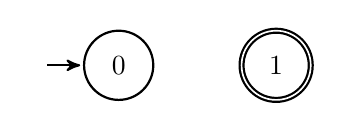
\begin{tikzpicture}[->,>=stealth',shorten >=1pt,auto,node distance=2cm,
    thick,base node/.style={circle,draw,minimum size=16pt}, real node/.style={double,circle,draw,minimum size=35pt}]

\node[initial,initial text={}, state]   (0)                     {0};
\node[state,accepting]                  (1)     [right of=0 ]   {1}          [above];

\end{tikzpicture}

对于正规式$\epsilon$,等价的NFA为:

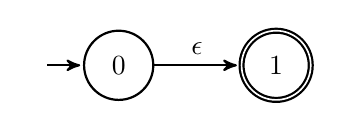
\begin{tikzpicture}[->,>=stealth',shorten >=1pt,auto,node distance=2cm,
    thick,base node/.style={circle,draw,minimum size=16pt}, real node/.style={double,circle,draw,minimum size=35pt}]

\node[initial,initial text={}, state]   (0)                     {0};
\node[state,accepting]                  (1)     [right of=0 ]   {1}          [above];
\path[]
(0) edge  node{$\epsilon$} (1);
\end{tikzpicture}

对于正规式a,等价的NFA为:

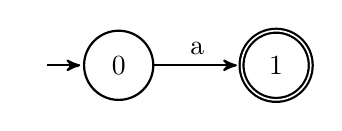
\begin{tikzpicture}[->,>=stealth',shorten >=1pt,auto,node distance=2cm,
    thick,base node/.style={circle,draw,minimum size=16pt}, real node/.style={double,circle,draw,minimum size=35pt}]

\node[initial,initial text={}, state]   (0)                     {0};
\node[state,accepting]                  (1)     [right of=0 ]   {1}          [above];
\path[]
(0) edge  node{a} (1);
\end{tikzpicture}

\noindent 复合正规表达式R转化为NFA

首先将复合正规表达式表示成如下扩广的状态转换图:

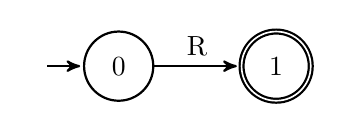
\begin{tikzpicture}[->,>=stealth',shorten >=1pt,auto,node distance=2cm,
    thick,base node/.style={circle,draw,minimum size=16pt}, real node/.style={double,circle,draw,minimum size=35pt}]

\node[initial,initial text={}, state]   (0)                     {0};
\node[state,accepting]                  (1)     [right of=0 ]   {1}          [above];
\path[]
(0) edge  node{R} (1);
\end{tikzpicture}

根据R,按照正规式的运算递归生成NFA M

若$R=R|S$将
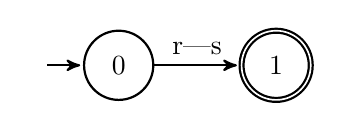
\begin{tikzpicture}[->,>=stealth',shorten >=1pt,auto,node distance=2cm,
    thick,base node/.style={circle,draw,minimum size=16pt}, real node/.style={double,circle,draw,minimum size=35pt}]

\node[initial,initial text={}, state]   (0)                     {0};
\node[state,accepting]                  (1)     [right of=0 ]   {1}          [above];
\path[]
(0) edge  node{r|s} (1);
\end{tikzpicture}
转换为
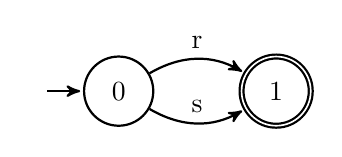
\begin{tikzpicture}[->,>=stealth',shorten >=1pt,auto,node distance=2cm,
    thick,base node/.style={circle,draw,minimum size=16pt}, real node/.style={double,circle,draw,minimum size=35pt}]

\node[initial,initial text={}, state]   (0)                     {0};
\node[state,accepting]                  (1)     [right of=0 ]   {1}          [above];
\path[]
(0) edge[bend left,above]  node{r} (1)
(0) edge[bend right,above]  node{s} (1);
\end{tikzpicture}

若$R=rs$
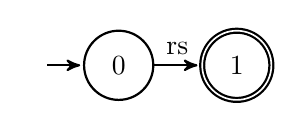
\begin{tikzpicture}[->,>=stealth',shorten >=1pt,auto,node distance=1.5cm,
    thick,base node/.style={circle,draw,minimum size=16pt}, real node/.style={double,circle,draw,minimum size=35pt}]

\node[initial,initial text={}, state]   (0)                     {0};
\node[state,accepting]                  (1)     [right of=0 ]   {1}          [above];
\path[]
(0) edge  node{rs} (1);
\end{tikzpicture}
转换为
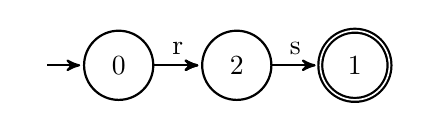
\begin{tikzpicture}[->,>=stealth',shorten >=1pt,auto,node distance=1.5cm,
    thick,base node/.style={circle,draw,minimum size=16pt}, real node/.style={double,circle,draw,minimum size=35pt}]

\node[initial,initial text={}, state]   (0)                     {0};

\node[initial,initial text={}, state]   (2)     [right of = 0]   {2};
\node[state,accepting]                  (1)     [right of = 2]   {1}      [above];
\path[]
(0) edge[above]  node{r} (2)
(2) edge[above]  node{s} (1);
\end{tikzpicture}

若$R=r^{*}$
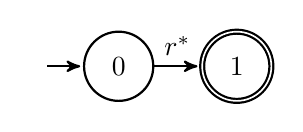
\begin{tikzpicture}[->,>=stealth',shorten >=1pt,auto,node distance=1.5cm,
    thick,base node/.style={circle,draw,minimum size=16pt}, real node/.style={double,circle,draw,minimum size=35pt}]

\node[initial,initial text={}, state]   (0)                     {0};
\node[state,accepting]                  (1)     [right of=0 ]   {1}          [above];
\path[]
(0) edge  node{$r^{*}$} (1);
\end{tikzpicture}
转换为
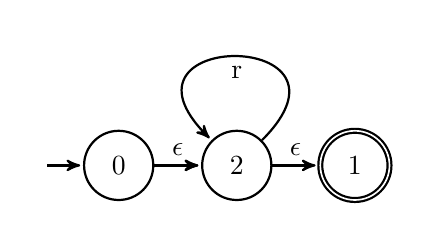
\begin{tikzpicture}[->,>=stealth',shorten >=1pt,auto,node distance=1.5cm,
    thick,base node/.style={circle,draw,minimum size=16pt}, real node/.style={double,circle,draw,minimum size=35pt}]

\node[initial,initial text={}, state]   (0)                     {0};

\node[initial,initial text={}, state]   (2)     [right of = 0]   {2};
\node[state,accepting]                  (1)     [right of = 2]   {1}      [above];
\path[]
(0) edge[above]  node{$\epsilon$} (2)
(2) edge[loop, below] node{r} (2) 
(2) edge[above]  node{$\epsilon$} (1);
\end{tikzpicture}

正规式$R=(r)$的NFA同正规式$R=r$的NFA相同

\noindent \textbf{从NFA到DFA}
\begin{enumerate}
\item 对任一NFA:M,总可构造一个DFA:M’,使$L(M’)=L(M)$成立
\item 状态s的$\epsilon$-闭包:定义为从s出发经过零个或多个$\epsilon -$转化能达到的状态的集合,并将这个集合记为$\hat{s}$
\item 状态集合S的$\epsilon -$闭包:定义为S中各个状态的$\epsilon$
\item 由NFA构造DFA的子集构造算法
\begin{itemize}
    \item 计算M初始状态$s_0$的$\epsilon -$闭包,令其作为$\overline{M}$的初始状态:$\overline{s_0}$
          $\overline{S}=\{\overline{s_0}\}, \overline{T}=\emptyset$
    \item 对于$\overline{s_i}=\{s_{i1}, s_{i2}, \dots , s_{im}\}$,标记$\overline{s_i}$,
          对于每个$a \in \sum$ 及 $\overline{s_i}=\{s_{i1}, s_{i2}, \dots , s_{im}\}$计算
          $s_{a}=\{t|T(s_{ij},a)=t, j \in[1\dots m]\}$, 计算$s_a$的$\epsilon -$闭包$\overline{s_a}$;
          令$\overline{S}=\overline{S} \cup \{\overline{s_a}\}$;
          令$\overline{T} = \overline{T} \cup \{ \overline{T}(\overline{s_i}, a) = \overline{s_a}\}$
    \item 重复步骤2直到$\overline{S}中没有未标记的状态$
    \item 令$\overline{A}=\{\overline{s_i}|\overline{s_i} \cap \neq \emptyset\}$
\end{itemize}
\end{enumerate}

\noindent \textbf{将DFA中的状态数最小化}
\begin{enumerate}
    \item 首先将状态集合S分为两个等价类:$A$及$S-A$
    \item 细分等价类:对于当前划分的某个等价类$K$,$s_{i},s_{j} \in K$满足如下条件
    \begin{itemize}
        \item $\exists a$, $s_1$或$s_2$中的一个无法识别$a$
        \item $\exists a$, $s_1,S_2$识别后到达的状态分别在目前划分的不同等价类中
    \end{itemize}
    那么将$K$就细分为两个等价类$K_i, K_j$,使$s_1 \in K_i, s_2 \in K_j$
    \item 递归上述步骤2中细分等价类的工作,知道所有等价类都不能再细分为止
\end{enumerate}

\noindent \textbf{用代码实现有穷自动机}
\begin{itemize}
\item 常见问题
\begin{enumerate}
    \item 错误问题:不在状态机中的均为错误状态
    \item 分隔符问题:需要回溯
    \item 最长匹配原则问题
\end{enumerate}
\item 逐个判断,不存储状态,到结束位置或错误位置跳出
\item 采用双层switch-case嵌套判断
\begin{enumerate}
    \item 第一层判断当前状态:state
    \item 第二层switch测试输入字符:ch.保存遇到该输入字符转换之后的状态,
    判断是否读下一个字符 
\end{enumerate}


\item 采用二维表(图)的形式用数据结构将转换结构存储起来为一个转化表
\end{itemize}

\section{上下文无关文法(2型文法)}

正规表达式的局限性:正规表达式不能用于描述配对(嵌套)的结构:$\{(n)^n | n > 1\}$;
正规表达式不能用于描述下述重复串:\{$wcw$|$w$是$a$和$b$形成的任意串\}

\noindent 上下文无关文法定义:$G$是一个四元组,即$G=(V_t, V_n, P, S)$
\begin{itemize}
    \item 终结符(或Token)集合$V_t$
    \item 非终结符集合$V_n$(与$V_t$不相交)
    \item 产生式或文法规则$A \rightarrow \alpha$形成的集合$P$,其中$A \in V_{n},\alpha \in {(V_{n} \cup V_{t})}^*$
    \item 开始符号S,其中$S \in V_n$
    \item 终结符和非终结符可以用单个字符表示,也可以用字符串表示
\end{itemize}

\noindent 推导与规约

直接推导或一步推导

直接推导就是产生式规则的一次运用,即用产生式的右部替换左部,记为$\Rightarrow$.

定义:若有$v,w$满足:$v=\gamma \alpha \delta, w=\gamma \beta \delta$,;其中$\alpha \rightarrow \beta$是文法$G$的产生式,
$\gamma \in (V_t \cup V_n)^*, \delta \in (V_t \cup V_N)^*$,则称$v$直接推导到$w$,记作$v \Rightarrow w$,也称$w$直接规约到$v$

若存在$w_0 \Rightarrow w_1 \Rightarrow \dots  \Rightarrow w_n (n > 0)$, 
用$w_0 {\Rightarrow} ^+ w_n$ 表示$w_0$到$w_n$ 经历一步或多步推导,称$w_0$推导出$w_n$ ,或$w_n$归约到$w_0$

若有$w_0 \Rightarrow ^* w_n$ ,或$w_0 = w_n$ ,则记为$w_0 \Rightarrow ^* w_n $,表示表示$w_0$到$w_n$零步或多步推导

句型和句子
\begin{itemize}
    \item 设$G=(V_N, V_t, P, S)$是一文法,且 $V=V_N \cup V_t$
    \item 若$S \Rightarrow ^* \alpha, \alpha \in V^*$,则称$\alpha$为文法$G$的句型;
    \item 若$S \Rightarrow ^+ \alpha, \alpha \in V_t^*$,则称$\alpha$为文法$G$的句子
\end{itemize}

\noindent 最左推导和最右推导

最左推导

对于文法$G[S],S \Rightarrow ^* \gamma$ 是一个最左推导是指:在由$S$推导$γ$的过程中,任何一步直接推导$\alpha \Rightarrow \beta$,都是用字符串$\alpha$中的最左非终结符对应的产生式规则进行推导,其中$\alpha, \beta$是句型

最右推导

$S \Rightarrow ^* \gamma$是一个最右推导是指:在由$S$推导$\gamma$的过程中,任何一步直接推导$\alpha \Rightarrow \beta$,都是用字符串$\alpha$中的最右非终结符对应的产生式规则进行推导,其中$\alpha, \beta$是句型。
最右推导也被称为规范推导,由规范推导所得的句型称为规范句型。

文法$G[S]$定义的语言$L(G)$为:
$L(G)$=\{$x|S \Rightarrow ^+ x$,其中$S$为开始符号,$x \in V_t^*$\} ,即语言是所有句子构成的集合;

上下文无关文法定义的语言称作上下文无关语言

递归产生式和递归文法

递归产生式:设给定2型文法$G=(V_N, V_t, P, S)$,若存在产生式$A \rightarrow xAy \in P$ ,
则称产生式A→xAy是递归产生式; $x,y \in (V_N \cup V_t)^*$
\begin{itemize}
    \item 若$x=\epsilon$且$y\neq \epsilon$,则称产生式$A \rightarrow Ay$是左递归产生式;
    \item 若$x \neq \epsilon $且$y=\epsilon$,则称产生式$A \rightarrow xA$是右递归产生式。
\end{itemize}


递归文法:若文法中至少存在一条递归产生式则称该文法是直接递归的文法;
若有$A \Rightarrow ^+ xAy$,$x,y \in (V_N \cup V_t)^*$则称文法为间接递归的文法。
对于文法中任一非终结符号,若能从它出发建立一个推导过程,在推导所得的符号串中又出现了该非终结符本身,则文法是递归
一般的文法都是递归的,文法$G$只有递归定义,$L(G)$中的句子才是无穷的


\noindent chomsky文法的分类
\begin{itemize}
    \item 0型文法:若文法$G$中任一产生式$\alpha \rightarrow \beta$,都有$\alpha \in (V_N \cup V_t)^+, \beta \in (V_N \cup V_t)^*$,则称$G$为0型文法
    \item 1型文法:若文法$G$中任一产生式$\alpha \rightarrow \beta$,都有$\alpha \in (V_N \cup V_t)^+, \beta \in (V_N \cup V_t)^*$,$|\beta| \geq |\alpha|$,仅仅$S \rightarrow \epsilon$除外,则称$G$为1型文法
    \item 2型文法:若文法$G$中任一产生式$\alpha \rightarrow \beta$,都有$\alpha \in V_N, \beta \in (V_N \cup V_t)^* $,则称$G$为2型文法,也称为上下文无关文法
    \item 3型文法:把右线性文法及左线性文法统称为3型文法或正规文法
    \begin{itemize}
        \item n若文法G中任一产生式$\alpha \rightarrow \beta$的形式都为$A \rightarrow aB$ 或 $A \rightarrow a$,其中$A \in V_N, B \in V_N, a \in V_t$则称$G$为右线性文法;
        \item 如果G中仅含有形如$A \rightarrow Ba$或 $A \rightarrow a$的产生式,则称G为左线性文法
    \end{itemize}
\end{itemize}


\noindent 分析树定义
\begin{itemize}
    \item 每个节点都用终结符、非终结符或$\epsilon$标出
    \item 根节点用文法的开始符号S标出
    \item 每个叶节点都用终结符或$\epsilon$标出
    \item 每个非叶节点都用非终结符标出
    \item 每一步直接推导对应一个子树:在分析树中,如果标记为$A \in V_N$的节点有n个标记为$X_1,X_2, \dots,X_n$的孩子,$X_i$可以是终结符也可以是非终结符,则文法$G$中有对应的产生式 $A \rightarrow X_1X_2\rightarrow X_n \in P$
\end{itemize}

\noindent 二义性文法

对于文法$G$,若存在某个句子$w \in L(G)$,w对应多个不同的最左推导(或最右推导),这类文法称为二义性文法

解决二义性文法的不确定性:修改文法;采用设置消除二义性的规则,如:优先权和结合性

二义性文法的充分条件:若一文法含有既是左递归又是右递归的文法符号,则G必定是二义性的
如$A \Rightarrow ^+ AvA v \in (V_N \cup V_T)^*$或 $A \Rightarrow ^+ A$ 或 $A \Rightarrow ^+ A\alpha$及$A \Rightarrow ^+ \beta A$


\section{语法分析}

\noindent 主要目的
\begin{itemize}
    \item 以词法分析程序输出的单词序列为输入,分析源程序的语法结构,判断是否为相应程序语言的合法程序
    \item 确定单词流中违反源语言语法结构规则的错误
    \item 分析结果:分析树或语法树
\end{itemize}

\noindent 主要步骤:
\begin{itemize}
    \item 对程序设计语言的语法规则进行形式化描述(2型文法)
    \item 根据语言的语法描述形式,定义各种基本语法结构的抽象语法树
    \item 选择一种合适的语法分析算法,并在分析程序中插入构造语法树等动作
\end{itemize}

\noindent 自上而下的语法分析算法

定义:已知文法$G[S]$,对任意输入串$w$,若从文法的开始符号$S$出发,能为$w$构造一个最左推导,则$w$是一个合法的句子,即$w \in L(G)$,否则$w$有语法错误
\\
\noindent 分析方法
\begin{itemize}
    \item 从文法开始符号S出发试图为输入符号串构造一个最左推导
    \item 构造最左推导的过程就是选择产生式和匹配符号串的过程
    \item 有时需要重复扫描词法分析输出的单词序列
\end{itemize}

\subsection{递归下降的方法}
递归下降分析方法是一种自上而下的语法分析方法,该方法执行一组递归函数判断输入的单词序列是否符合语法规则.

递归函数:为每一个产生式规则撰写一个函数,以产生式左部的非终结符作为函数的名字,根据产生式规则的右部撰写函数体.
遇到总结符,匹配并读取下一个单词;遇到非终结符,调用该非终结符所在产生式对应的函数.

\noindent EBNF文法规则
\begin{itemize}
    \item 选择:采用 [] 包含起来,表示可选项
    \item 重复
    \begin{itemize}
        \item $A \rightarrow A\alpha | \beta$(左递归) $\Rightarrow  \ A \rightarrow \beta\{\alpha\}$ 
        \item $A \rightarrow \alpha A| \beta$(右递归) $\Rightarrow  \ A \rightarrow \{\alpha\}\beta$ 
    \end{itemize}
    \{\}表示其中的内容重复n次($n \geq 0$),写递归下降语法分析程序时可将花括号表示的重复部分翻译成循环代码
\end{itemize}

\noindent 会遇到的问题

\begin{itemize}
    \item 间接递归的文法$\Rightarrow$进行等价改造
    \item 对于两个或多个文法规则的选项,在一次判断决定使用那一个文法而不是去回溯判断
    \item 在递归下降分析程序中,应该增加代码以实现保存语法分析结果的功能
    \begin{itemize}
        \item 构造相应的语法数节点
        \item 保持运算的结合性
        \item 计算表达式值
    \end{itemize}
\end{itemize}

分析树与抽象语法树

\subsection{LL(1)分析(自上而下分析)}
\noindent 名词解释
\begin{itemize}
   \item 第1个“L”指的是由左向右地处理输入;
   \item 第2个“L”指的是它为输入串找出一个最左推导;
   \item 括号中的数字1意味着它使用输入单词序列中的一个单词预测分析的动作。
\end{itemize}

\noindent 构造最左推导的语法分析程序要解决的问题
\begin{itemize}
    \item 定位当前句型进行下一步推导的非终结符
    \item 选择产生式
    \item 符号串的替换
\end{itemize}

\noindent\textbf{LL(1)分析的基本方法}

通过栈来“记忆”针对当前句型中的哪一个非终结符进行推导,首先将文法的开始符号S入栈;

如果栈的顶部是非终结符A,则利用A对应的某个文法规则$A \rightarrow \alpha$将栈顶部的非终结符A(出栈)替换成串$\alpha$(将串$\alpha$自右至左入栈)。

如果栈的顶部是终结符a,则查看已推出的终结符是否与当前输入单词匹配?(如匹配则出栈)。

构造一个非终结符和终结符索引的二维表格$M[N,T]$,通过表格指出用哪一个产生式进行进行下一步推导,其中N是非终结符的集合,T是终结符的集合。

\noindent\textbf{构造LL(1)分析表}


文法符号X的\textbf{First(X)集合}

若$X$是终结符或$\epsilon$,则$First(X)={X}$

若$X$是非终结符,则$X$对应的每个产生式$X \rightarrow X_1X_2 \dots X_n$
$First(X)$包括$First(X₁)-\{\epsilon\}$

若对于某个$i<n$,所有的集合$First(X_1),\dots,First(X_i)$都包括了$\epsilon$,则$First(X)$也包括$First(X_{i+1})-\{\epsilon\}$

若所有集合$First(X_1),\dots,First(X_n)$包括了$\epsilon$,则$First(X)$也包括$\epsilon$

\noindent\textbf{求Follow集合}

给出一个非终结符A,集合Follow(A)是由终结符组成,此外可能还有$,定义如下所示:
若A是开始符号,则Follow(A)包含$
若存在产生式B→αAγ,则Follow(A)包含First(γ)-{ε}
若存在产生式B→αAγ,且ε在First(γ)中,则Follow(A)包含Follow(B)
求解Follow(A),考虑A出现在哪些产生式右部。Follow集仅针对非终结符,并且不包含ε

\noindent\textbf{构造LL(1)分析表}

\noindent 构造方法:

分析表以非终结符作为行索引,以终结符作为列索引,分析表的元素位置存储产生式,为每个非终结符A和它对应的产生式$A \rightarrow \alpha$重复以下步骤

对于$First(\alpha)$中的每个终结符a,都将$A \rightarrow \alpha$添加到$M[A,a]=A \rightarrow \alpha$

\begin{center}
\begin{tabular}{|c|c|c|}
    \hline 
    \  & a & \  \\
    \hline 
    A & $A \rightarrow \alpha$ & \ \\ 
    \hline
\end{tabular}
\end{center}

即当当前分析栈的栈顶符号为$A$时,而当前词法分析输入单词为$a$时,按照产生式$A \rightarrow \alpha$进行推导

若$\epsilon$在$First(\alpha)$中,则对于$Follow(A)$的每个元素a(或者\$),都将$A \rightarrow \alpha$添加到$M[A,a]$中。即在此情况下按产生式$A \rightarrow \alpha$进行推导

\begin{center}
    \begin{tabular}{|c|c|c|}
        \hline 
        \  & a & \  \\
        \hline 
        A & $A \rightarrow \alpha$ & \ \\ 
        \hline
\end{tabular}
\end{center}

例如$bAa\dots \Rightarrow b\alpha a\dots ^* \Rightarrow b\epsilon a\dots \Rightarrow ba\dots$

所有没有定义的元素位置$M[A,a]$标上“出错标志”。

文法G相关的$LL(1)$分析表的每个项目中至多只有一个产生式,则该文法就是$LL(1)$文法。
含有左递归和左公共因子的文法不是LL(1)文法

\noindent 消除左递归
\begin{enumerate}
    \item 简单直接左递归的消除$A \rightarrow A\alpha, A \rightarrow \beta$ 将文法重写为$A \rightarrow \beta B, B \rightarrow \alpha B| \epsilon$
    \item 多项式直接左递归的消除 $A \rightarrow A{\alpha}_1|A{\alpha}_2| \dots A{\alpha}_n|{\beta}_1|{\beta}_2| \dots |{\beta}_m$消除左递归重写文法为
          $A \rightarrow {\beta}_1B|{\beta}_1B|\dots|{\beta}_mB, B \rightarrow {\alpha}_1B|{\alpha}_2B|\dots|{\alpha}_nB|\epsilon$
\end{enumerate}

\noindent 提取左因子

若有产生式$U \rightarrow xy|xw|\dots|xz$,则提取左公共因子并用EBNF表示为:$U \rightarrow x(y|w|\dots|z)$再引入另一个非终结符V,将产生式变为$U \rightarrow xV, V \rightarrow y|w|\dots|z$
若在$y,w,\dots,z$中仍然有坐公共因子,可以再次提取。若有$U \rightarrow xy|x$则提取后$U \rightarrow x(y|\epsilon)$

\subsection{自下而上的语法分析}
\noindent 概述
\begin{itemize}
\item 从输入单词序列开始,自左至右逐步进行规约(最右推导的逆过程,称为规范规约),试图将器规约为文法的开始符号
\item 从输入单词序列开始,以单词作为语法树的叶节点,自底向上构造语法分析的结果——语法树
\item 自左至右规约是最右规范推导的逆过程,称之为规范规约
\item 自下而上语法分析的每一步,都是从当前串中选择一个子串,将它规约到某个非终结符号
\item 每次规约的子串称为句柄
\end{itemize}

\noindent 句柄

句型$\alpha \beta \delta$的直接短语:若有$S \Rightarrow ^* \alpha A \delta \rightarrow \alpha \beta \delta, \alpha, \beta, \delta \in (V_N \cup V_t)^*、A \in V_N$
则称β是句型αβσ相对于非终结符A的直接短语

句型$\alpha \beta \delta$的句柄:句型的最左直接短语(在规范推导中,最先被规约的子串),称为句型的句柄

\subsubsection{LR(k)分析}

\noindent 优点
\begin{itemize}
    \item 应用面广:能够通过$LR$分析程序识别所有采用上下文无关文法描述的程序设计语言的语法结构
    \item 能有效实现:是无回溯的移进-规约方法
    \item 容易查错:LR分析器能够及时发现语法错误和准确指出错误位置
\end{itemize}

\noindent 部分名词解释
\begin{itemize}
    \item L是指自左向右分析输入单词序列
    \item R是指分析过程都是构造最右推导的逆过程
    \item 括号中的k是指在决定当前分析动作时向右看的单词个数
    \item 符号前缀的定义:符号串的前缀是指从符号串的尾部删去若干个(包括0个)符号之后所剩余的部分
    \item 活前缀和可归前缀
    \begin{itemize}
        \item  设有文法$G[S]$,若$S \Rightarrow ^*\alpha A \omega \Rightarrow \alpha \beta \omega$是文法$G$的一个规范推导,$(\alpha ,\beta \in (V_N \cup V_t)^+, \omega \in V_t^*, A \in V_N)$;
        $\alpha \beta$的一个前缀称为文法$G$的一个活前缀;
        $\alpha \beta$称为文法$G$的可归前缀
        \item 在规范规约的过程中,自左向右分析输入串的任何时刻,在符号栈中的符号串均为规范句型的活前缀
        \item 如果符号栈的内容是当前句型的可归前缀,那么栈顶已经形成当前句型的句柄,进行规约,否则继续移进
    \end{itemize}
\end{itemize}

\noindent 需要解决的主要问题
\begin{itemize}
    \item 如何识别符号栈中栈顶的符号组成的符号串是否是可归前缀,是可归前缀就规约,否则移进
    \item 分析表指导,分析表如何构造
    \begin{itemize}
        \item 求文法中的所有可归前缀
        \item 识别可归前缀和活前缀
        \item 分析表的构造
    \end{itemize}
\end {itemize}

\noindent\textbf{识别可归前缀和活前缀}

\noindent 将所有的文法用状态机表示,先表示为NFA再转化为DFA
\begin{itemize}
    \item 中间状态为活前缀识别态(移进)
    \item 所有终态都是可归前缀的识别态,此时分析栈中形成句柄(规约)
    \item 带$(*)$的状态为唯一的句子识别态,此次规约到开始符号
\end{itemize}

\noindent\textbf{分析表的构造}
\begin{itemize}
    \item 分析表由动作表和状态转化表组成
    \begin{itemize}
        \item 动作表(Action)以一个二维数组表示,列代表识别活前缀的状态(i),行代表当前的输入符号(a),数组元素Action[i,a]表示所执行的动作(移进,规约,接受,报警)
        \item 状态转化表用一个二维数组表示,列代表识别活前缀的状态,行代表文法符号,数组元素表示为当前识别活前缀的状态为i,面对文法符号为X时,应转为新的状态Goto[i,X]
    \end{itemize}
    \item 分析表的动作
    \begin{itemize}
    \item 移进:输入符号进符号栈
    \item 归约:用相应的产生式进行归约
    \item 接受:当文法符号归约到只剩下开始符号,且输入串结束时(当前输入为\$),分析成功
    \item 报警:当状态栈顶为某一状态下,出现了不该出现的文法符号时报错。
    \end{itemize}
\end{itemize}

LR分析算法的主要过程


\begin{center}
\begin{tikzpicture}[node distance = 2cm, auto]
    % Place nodes
    \node [block] (main) {总控程序};
    \node [block, above of=main,text width=4cm] (input) {$a_1a_2\dots a_ia_{i+1}\dots a_n$\$};
    \node [block, left of=main, left = 2cm] (stack) {状态栈与符号栈};
    \node [block, right of=main, right = 2cm] (output) {输出};
    \node [block, below of=main, left = 1cm] (action) {动作表};
    \node [block, below of=main, right = 1cm] (state) {状态转化表};
    % Draw edges
    \path [line] (main) -- (action);
    \path [line] (main) -- (state);
    \path [line] (main) -- (input);
    \path [line] (main) -- (output);
    \path [line] (main) -- (stack);
\end{tikzpicture}
\end{center}

在总控程序的控制下,从左到右处理词法分析输入串,根据分析栈和输入符号的情况,查分析表确定分析动作

分析栈包括文法符号栈$X[i]$和相应的状态栈$S[i]$两部分(状态是指识别活前缀的自动机状态)。

分析表是LR分析器的核心,它包括动作表(Action)和状态转换表(Goto)两部分。

根据识别文法所有活前缀和可归前缀的有限自动机,可以构造分析表来指导移进-规约动作。

\subsubsection{LR(0)分析算法(不存在移进-规约冲突和规约-规约冲突)}

\noindent 项目的定义

对于文法$G$,其产生式的右部添加一个特殊符号".",就构成文法的一个$LR(0)$项目,简称项目.

若$A \rightarrow \beta \gamma$是产生式,其中$\beta$和$\gamma$是任意符号串(包括空串),那么$A \rightarrow \beta . \gamma$就是$LR(0)$项目,
每个项目中圆点的左部表示在分析过程中要用该产生式归约时,句柄已识别的部分(进入符号栈),右部表示等待识别的部分

\noindent 构造识别活前缀的NFA

NFA的构造原则:为了确保有唯一的接受项目,首先扩广文法$G$为$G'$,引进一新的产生式$S' \rightarrow S$,$S'$是新增加的非终结符作为G'的开始符
\begin{itemize}
    \item NFA的状态集:每个项目对应一个NFA状态,所有项目对应的状态的集合;
    \item 输入字符集合:包括终结符、非终结符和$\epsilon$
    \item 初态:对于文法$G[S]$的扩广文法$G[S']$,有项目$S' \rightarrow .S$,由于$S'$仅在第一个产生式的左部出现,规定它为初态
    \item 终态:对于扩广文法$G[S']$,有项目$U \rightarrow u.$(即圆点在最后的项目),作为NFA的终态
    \item 转化函数$f$:若文法中有项目$i$为:$X \rightarrow x_1 \dots x_{i-1}.x_i \dots x_n$;项目$j$为:$X \rightarrow x_1\dots x_i .x_{i+1} \dots x_n$;
    则有转化函数$GO(i,x_i)=j$
    若$x_i$为非终结符号,则还有转化函数$GO(i,\epsilon)=k$,项目$k$为:$x_i→.\beta$
\end{itemize}

\noindent 构造识别活前缀的DFA

基于闭包函数$CLOSURE(I)$以及转移函数$GO(I,x)$构造识别活前缀的DFA

$CLOSURE(I)$的定义:扩广文法$G'$的一个$LR(0)$项目集合$I$的闭包函数
\begin{enumerate}
    \item 令$CLOSURE(I)=I$
    \item 令项目${A \rightarrow \alpha .B \beta} \in CLOSURE(I), {B \in V_N}$,则$CLOSURE(I)=CLOSURE(I)\cup \{B \rightarrow.\gamma\}$
    \item 重复步骤2直至$CLOSURE(I)$不增加新的项目为止
\end{enumerate}

$GO(I,x)$的定义:$GO(I,x)=CLOSURE(J)$,其中:J是I识别符号x后所到达的项目集,$J=\{A \rightarrow \alpha x.\beta|A \rightarrow \alpha x. \beta \in I\}$
\\

\noindent 构造识别活前缀的DFA步骤
\begin{enumerate}
    \item 令项目集$CLOSURE({S'\rightarrow .S})$为DFA的初态
    \item 输入字符集合:包括终结符、非终结符
    \item 设$I$是$DFA$中一个已存在的状态(项目集),若存在$A\rightarrow \alpha x. \beta \in I$,则对$x \in V_t \cup V_N$
    \begin{itemize}
        \item 计算$GO(I,x)=CLOSURE(J)$,将项目集$CLOSURE(J)$作为DFA的一个新状态加入DFA的状态集
        \item 同时将转移函数$GO(I,x)=CLOSURE(J)$作为DFA的转移函数
    \end{itemize}
    \item 重复2直至DFA的状态集中不产生新的状态为止
    \item 含有项目$U \rightarrow u.$的项目集,作为DFA的终态
\end{enumerate}


\noindent LR(0)分析表的构造
\begin{itemize}
    \item 设状态$i,j$,若有$GO(i,x)=j$,对于状态$i$中的项目$A \rightarrow \alpha x.\beta$,若$x\in V_t$,则置$Action[i,x]=S_j$;若$x \in V_N$,则置$Goto[i,x]=j$;
    \item 对于终态i中的项目$A \rightarrow \alpha$.,若$A \rightarrow \alpha $是G中第k个产生式,则对所有输入符号$x \in V_t$(包括\$),均置$Action[i,x]=r_k$
    \item 若终态i中含项目S'→S.则置Action[i,\$]=acc(\$表示输入串结束符)
    \item 其他情况均置错
\end{itemize}

\noindent \textbf{LR(0)分析算法}
\begin{itemize}
    \item 将输入串的左边界(\$)进符号栈和初始状态0进入状态栈
    \item 根据状态栈栈顶状态i和当前输入符号a查Action表进行如下工作
    \begin{itemize}
        \item 移进:若$Action[i,a]=S_j$,当前输入符号$a$进符号栈,并将输入符号所对应的新的状态$j$进状态栈,继续处理下一个输入符号
        \item 归约:若$Action[i,a]=r_j$,按指定产生式进行归约,假设产生式右部的符号串长度为n,则
        \begin{itemize}
            \item 符号栈栈顶的n个符号为句柄,所以符号栈栈顶n个符号出栈,同时,状态栈栈顶的n个元素也出栈
            \item 归约后的文法符号A(非终结符)进符号栈
            \item 假设当前状态栈栈顶为j,若Goto[j,A]=k,则将文法符号A所对应的新状态k进状态栈
            \item 接受:若动作表中对应“acc”,则分析成功;
            \item 出错:若动作表中对应空白,则报告错误信息
        \end{itemize}
        \item 重复步骤2直到接受或出错为止
    \end{itemize}
\end{itemize}

项目的分类:项目分类的原则是根据圆点所在位置和圆点之后是终结符还是非终结符进行的
\begin{itemize}
    \item 移进项目:圆点之后为终结符的项目,$A\rightarrow \alpha.a\beta ,\alpha ,\beta \in V^*,a \in V_t$,它对应的状态为移进状态
    \item 待约项目:圆点之后为非终结符的项目,$A \rightarrow \alpha.B\beta ,\alpha , \beta \in V^*, B \in V_N$,它对应的状态为待约状态
    \item 归约项目:圆点之后没有符号(圆点在最后)的项目,$A \rightarrow \alpha . \alpha \in V^*$,它对应的状态为归约状态
    \item 接受项目:对于扩广文法$G[S']$,有项目$S' \rightarrow S$.它是一个特殊的归约项目,称它为接受项目,它所对应的状态为接受状态
\end{itemize}

\noindent LR(0)文法的定义

项目集的相容性:在一个项目集(对应DFA的一个状态)中,若能满足下述条件,则称该项目为相容的项目集
\begin{itemize}
    \item 移进项目和归约项目不并存,否则是移进-归约冲突
    \item 多个归约项目不存在,否则称归约-归约冲突
\end{itemize}

LR(0)文法:若一个文法G的任一项目集中的所有项目都是相容的(即LR(0)分析表表项的元素至多只有一个),则称文法G为LR(0)文法


\subsubsection{SLR(1) (不存在规约-规约冲突有可能存在移进-规约冲突)}

在SLR(1)文法中,向右看一个符号,所以属于LR(1)方法,而它仅在发生冲突时才向右看一个符号

SLR(1)文法于LR(0)文法识别齐活前缀项目集合的DFA一样,区别在于它们构造分析表的规则不一样

任意文法G[S]的SLR(1)分析表的构造规则如下:

\begin{itemize}
    \item 设状态$j$为状态$i$输入符号$x$后到达的状态,即$GO(i,x)=j$,对于状态i中的项目$A \rightarrow \alpha .x\beta$,若$x \in V_t$,则置$Action[i,x]=S_j$;若$x \in V_N,则置Goto[i,x]=j$;
    \item 对于状态$i$中的归约项目:$A\rightarrow \alpha . \in i$ 若$A \rightarrow \alpha$为文法的第$j$个产生式,则对于任意输入符号$a$,$a \in Follow(A)$,则置$Action[i,a]=r_j$
    \item 若$S \rightarrow \alpha. \in i$,则置$Action[i,\$]=acc$(S为开始符号)
    \item 其他情况均置出错
\end{itemize}

\subsubsection{LR(1):在SLR(1)中非终结符的Follow集和和First集合有交集,通过LR(1)来解决问题}

LR(1)项目:在LR(0)项目中放置一个向右搜索符号a,成为LR(1)项目:$[A\rightarrow \alpha .\beta, a]$

LR(1)分析过程中的每一个状态,就是包含若干LR(1)项目的一个LR(1)项目集

构造LR(1)项目集合的DFA的算法于LR(0)类似,也需要求两个函数CLOSURE和GO

构造闭包函数
\begin{itemize}
    \item $CLOSURE(I)=I$;
    \item 若存在$[A \rightarrow \alpha .B \beta ,a] \in CLOSURE(I), B \in V_N$, 则$CLOSURE(I)= CLOSURE(I)\cup \{[B \rightarrow .\gamma, b]\}$ ,其中 $b \in First(\beta \alpha)$
    \item 重复步骤2直至CLOSURE(I) 不增加新项目为止。
\end{itemize}

状态转移函数$GO(I,x)$:$GO(I,x)=CLOSURE(J)$,其中J是I识别符号x后所到达的项目集,后跟符号不变
$J=\{[A \rightarrow \alpha x.\beta,a]|[A \rightarrow \alpha .x\beta ,a]\in I\}$

基于闭包函数和转移函数构造文法$G'$的$LR(1)$项目集的识别文法活前缀的DFA,算法如下:

从初始状态出发,如果.后面的一位始非终结符$A\gamma$,则将该非终结符可以推出的状态加入,后跟符号是初始状态的后跟符号加上First($\gamma$后跟符);如果.后为总结符,则直接将.往后移,后跟符号不变
\begin{itemize}
    \item 令DFA的初态为项目集$CLOSURE({S' \rightarrow .S,\$})$
    \item 设I是一个DFA中的状态(已存在的项目集),对$x \in V_N \in V_t$
    \item 产生新的项目集$CLOSURE(J)$作为DFA的一个新状态加入DFA的状态集中:$GO(I,x)=CLOSURE(J)$
    \item 同时将转移函数$GO(I,x)=CLOSURE(J)$作为DFA的转化函数
    \item 重复2直至DFA中不产生新的项目集为止
    \item 含有项目$U \rightarrow u.$(即圆点在最后的项目)的项目集,作为DFA的终态
\end{itemize}

\noindent LR(1)分析表构造规则
\begin{itemize}
    \item 对于$[A \rightarrow \alpha .x \beta,a] \in$ 状态$i$,且$GO(i,x)=j$
    \item 若$x \in V_t$,则置$Action[i,x]=S_j$
    \item 若$x \in V_N$,则置$Goto[i,x]=j$
    \item 对于$[A \rightarrow \alpha.,a]∊$ 状态$i$,若$A \rightarrow a$是文法的第$j$个产生式,则置$Action[i,a]=r_j$
    \item 对于$[s \rightarrow \alpha .,\$]∊$状态$i$,则$action[i,\$]=acc$
    \item 其他情况置错
\end{itemize}

\subsubsection{LALR(1)}
LR(1)缺点:分析表状态数过大,使分析的效率降低

LALR(1)分析(Lookahead-LR)的基本思想是将LR(1)项目集中的同心集合并,将其压缩为较小的DFA,若压缩过程中未带来新的冲突,则分析表可大大地简化(状态数与SLR(1),LR(0)的DFA相同)

LALR(1)项目集(状态)通过同心集合并构造(同心集不会产生新的移进-归约冲突有可能产生新的归约-归约冲突)
\begin{itemize}
    \item 同心集:LR(1)的两个项目集的LR(0)项目全部相同,则称两个LR(1)项目集具有相同的心,具有想同心的项目集称为同心集
    \item 同心集合并
    \begin{itemize}
        \item 相同的心(LR(0)项目)不变
        \item 合并后项目集的搜索符等于合并前LR(1)项目搜索符的并集
    \end{itemize}
    \item 若合并同心集后项目集无分析动作冲突,或构造的LR分析表无冲突,则此表称为LALR(1)分析表
\end{itemize}


\section{语义分析}
静态语义:在编译阶段能够检查的语义

动态语义:在目标程序运行阶段能够检查的语义

任务
\begin{itemize}
    \item 计算各类语法成分的语义信息(属性信息)
    \begin{itemize}
        \item 一般将收集的语义信息存放到相应的信息表中,在编译程序中符号表是用来存放源程序中标示符相关属性(语义)信息的一种信息表
    \end{itemize}
    \item 静态语义检查
    \begin{itemize}
        \item 类型检查:指类型相容问题的检查,如果操作符作用于不同的操作数,则编译器应该报错
        \item 上下文有关问题的检查:当某个对象出现时,要求它必须在前面的某个适当的位置已经出现过
        \item 唯一性检查:要求某个对象只能被定义一次
        \item 控制流检查:引起控制流从某个结构中跳转出来的语句,必须能够决定控制流转向的目标地址
        \item break和continue语句是否在循环结构中
        \item 对于一个方法调用,实际参数的类型和实际参数的个数是否于方法的声明的参数特征相符
        \item 数组下标应用是否超出范围
        \item 数组下标是否是整数
    \end{itemize}
\end{itemize}

属性和属性文法

属性文法是一个三元式:A=(G,V,F)
\begin{itemize}
    \item G是一个上下文无关文法
    \item V是一个属性的有限集合
    \begin{itemize}
        \item 每个文法符号(总结符或非总结符)都有一个属性集(语义信息)
        \begin{itemize}
            \item 如果X是一个文法符号,与X关联的属性a的指记作X.a
            \item 文法符号关联的属性可以代表
            \begin{itemize}
                \item 变量的数据类型
                \item 表达式的值
                \item 存储器中变量的位置
                \item 程序的中间或目标代码片段
                \item 数的有效位数
            \end{itemize}
        \end{itemize} 
    \end{itemize}
    \item F是一个与属性有关的语义规则的有限集合:每个产生式都有一个与文法符号属性相关的语义规则集合。对于上下文无关文法中的任一产生式
          $X_0 \rightarrow X_1X_2\dots X_n$,其语义规则定义格式如下:
          $X_i.a_j=f_{ij}(X_0.a_1,\dots,X_0.a_{k}, X_1.a₁,\dots,X_1.a_k,\dots,X_n.a_1,\dots,X_n.a_k)$,
          其中$a_1,\dots,a_k$是与各文法关联的属性集合;$f_{ij}$是一个数学函数,表示文法符号$X_i$的第$j$个属性$a_j$是如何计算得到的
    \item   产生式的语义规则是产生式中相关文法符号属性值的等式
\end{itemize}

属性$a_1,\dots,a_k$的属性文法是文法所有产生式的语义规则的集合,一般将属性文法写成表格形式,每个产生式用相应语义规则列出

\noindent 属性文法的作用
\begin{itemize}
    \item 根据已求得的各产生式的语义规则,遍历语法分析的结果--语法树或分析树,计算任意句子的推导过程中各文法符号对应的属性值
    \item 根据属性值分析相关语义,或者将属性值存储在符号表中,以供编译的后续阶段使用
\end{itemize}

属性文法的求解方法
\begin{itemize}
    \item 给出一个句子最左推导对应的分析树,而且该句子的推导过程中基本涵盖各种语法规则的运用
    \item 根据该句子的分析树和已知文法符号的属性值,概括出各节点属性值的计算规则,将该计算规则作为节点对应的产生式的语义规则,最后得到属性文法
\end{itemize}

合成属性:如果给定一个产生式$A \rightarrow X_1X_2\dots X_n$,相关属性等式满足:$A.a=f(X_1.a_1,\dots,X_1.a_k \dots,X_n.a_1,\dots,X_n.a_k)$,则属性a是合成的,从语法分析树角度看,如果一个节点(文法符号)的某一属性值由其子节点的属性值来计算,则称该属性为合成属性

一个属性文法中所有的属性都是合成的,就称作S-属性文法

合成属性的计算:给定由语法分析程序构造的分析树或语法树,S-属性文法的属性值可以通过对树进行简单的自底向上后后序遍历来计算

\noindent{继承属性}
\begin{itemize}
    \item 从语法分析树角度看,一个节点的某一属性值是由父节点和/或兄弟节点的属性值来计算
    \item 继承属性的计算可以通过对分析树或语法树的前序遍历或中序遍历的组合来进行
    \item 在包含合成和继承属性的属性文法中,如果合成属性依赖于继承属性以及其他合成属性,但继承属性不依赖于任何其他合成属性,那么就可能在分析树或语法树的一遍遍历中计算所有的属性
\end{itemize}

属性计算方法
\begin{itemize}
\item 语法分析结果:抽象语法树遍历的属性计算方法.假设语法分析的结果--分析树或语法树已经建立来。并且树中已带有终结符的相应属性,可以以某种次序遍历语法树,直至计算出所有属性,如果需要的话,可使用多次遍历
\item 一遍语法分析的处理方法:语法分析时属性的计算。与树遍历的属性计算文法不同,一遍语法分析的处理方法是在语法分析的同时计算属性值,而不是语法分析构造语法树之后进行属性的计算
\item 语法分析时属性的计算.语法分析时属性的计算方法与语法分析器的相互作用,它与下面两个因素密切相关:
所采用的语法分析方法;属性的计算次序,语法分析方法都要求从左向右遍历分析树进行赋值
\end{itemize}

L-属性:对每个继承属性a𝒿和每个文法规则$X_0 \rightarrow  X_1X_2 \dots X_n$,  $a_j$的相关等式都有以下形式:$X_i.a_j=f_{ij}(X_0.a_1,\dots,X_0.a_k,X_{i-1}.a_1,\dots,X_{i-1}.a_k)$
即在$X_i$处$a_j$的值只依赖于文法规则中$X_i$左边出现的符号$X_i, \dots , X_{i-1} $的属性

给定一个L-属性文法,如果其继承属性不依赖于合成属性,递归下降的分析程序可以对所有的属性赋值

对于S-属性(合成属性),通常使用自底向上的分析方法,在建立每一个节点处使用语义规则来计算合成属性值

许多属性值相同,或者仅仅在计算其他属性值是临时使用,则可将属性作为函数的参数或返回值,而不是把它们作为字段存储在语法树节点的记录结构中

符号表:存储函数、变量、常量以及数据类型等标识符相关的信息
\begin{itemize}
    \item 作用
    \begin{itemize}
        \item 在词法分析、语法分析和语义分析的过程中收集有关标识符的属性,并存在符号表中
        \item 作为进行语法和语义的合法性检查的依据:同一个标识符可能在程序的不同地方出现,需要检查标识符在上下文中的一致性和合法性
        \item 作为目标代码生成阶段地址分配的依据:每个变量在目标代码生成是都需要确定其对应的存储地址,编译程序在完成来对变量的地址分配后,将其存于符号表中,可以通过符号表获取每个变量对应的存储地址
    \end{itemize}
    \item 内容:一个符号表包括若干登记项,每一项除来包括符号的名字外,还要填入其他信息(属性域),即每一项的形式为名字栏+属性栏
    \begin{itemize}
        \item 属性栏一般由若干子栏组成,用来记录与该项目名字相对应的各种属性之值和特征
        \item 每个名字的属性信息包括:名字的种类、类型、出现的特征、分配的存储单元地址,与该名字的语义有关的其他信息
    \end{itemize} 
    \item 对符号表的操作
    \begin{itemize}
        \item 增:向表中填入一个新的名字
        \item 删:从表中删除一个或一组无用的项
        \item 改:对给定名字,在表中填写或更新它的某些信息
        \item 查:对给定的名字,判定此名字是否已在表中
        \item 查:对给定名字,访问它在表中的某些相关信息
    \end{itemize}  
    \item 符号表的数据结构
    \begin{itemize}
        \item 线性链表
        \item 平衡二叉树
        \item 哈希表(数组加链表)
        \begin{itemize}
            \item 将标识符名转化成0...size-1范围内的一个整数
            \item 将字符串中的每个字符转化成一个非负整数
            \item 将这些整数用一定的方法组合形成一个整数
            \item 把整数调整到0...size-1范围内
        \end{itemize}
    \end{itemize}  
    \item 变量申明对符号表行为的影响.变量声明对符号表实现的影响是声明的作用域。编程语言中的作用域规则变化很广,采用下述公共的规则
    \begin{itemize}
        \item 使用前声明:它允许符号表在语法分析期间建立,当在代码中遇到对名字的引用时进行查找;如果查找失败,就出现声明错误,编译器给出相应的出错消息
        \item 块结构:一种语言是块结构的,如果它允许在一个作用域块的内部嵌入其他块.如果一个块中声明的作用域限制在本块以及本块包含的其他块,一般服从最近嵌套规则,即为同一个名字给定几个不同的说明,被引用的说明是最接近引用的那个嵌套块
        \item 实现嵌套作用域的方案一
        \begin{itemize}
            \item 为了实现嵌套作用域和最近嵌套规则,符号表插入操作不必改写前面的声明,再插入新的声明即可,这样查找操作只能找到名字最近插入的声明
            \item 删除操作不应该删除与这个名字相应的所有声明,只需删除最近的一个,而显示前面任何的声明
        \end{itemize}
        \item 实现嵌套作用域的方案二:
        为每个作用域建立一个新的符号表,再从内到外把它们链接在一起,这样如果查找操作在当前表中没有找到名字,就自动用附上的表继续搜索

    \end{itemize}
\end{itemize}

\noindent 数据类型和类型检查
\begin{itemize}
    \item 由编译器完成的检查称为静态检查
    \item 在目标程序运行时完成的检查则称为动态检查,原则上,如果目标代码将每个元素的类型和其值保存在一起,则任何检查都可以动态完成
    \item 类型检查
    \begin{itemize}
        \item 类型检查器将验证结构的类型是否与上下文所期望的类型匹配
        \item 类型检查器必须能够验证指针地址访问只作用于指针,下标运算只作用与数组,用户自定义的函数只能用于有正确参数个数及参数类型等情况
    \end{itemize}
\end{itemize}

\section{代码生成}

中间代码生成的主要步骤
\begin{itemize}
    \item 抽象语法树的结构
    \item 中间代码三地址码规范
    \item 三地址码生成统一的方案
    \item strval更新
    \item 后序递归遍历
\end{itemize}

中间代码
\begin{itemize}
    \item 编译程序的任务是把源程序翻译成等价的目标程序。所谓等价,是指两者之间的语法结构不同,但它们表述的功能和结果是完全相同的,即语义相同
    \item 中间代码,也称中间语言,是复杂性介于源程序和目标程序之间的一种机内表达形式,它是编译程序产生的中间临时结果。中间代码程序同源程序和目标程序的关系也同样是等价的,即结构不同,但语义相同。
    \item 中间代码优点
    \begin{itemize}
        \item 使编译程序的算法清晰,便于分工、修改、维护和移植等;
        \item 中间代码使编译器更容易重定向:不同机器上的编译器可以在已有前端的基础上附加一个适合这这台新机器的后端来生成;
        \item 可以在中间代码上进行与机器无关的代码优化,优化过程实际上是对程序的操作过程,对程序进行操作必须首先把程序转换成其结构便于操作的数据,而中间代码正是为此设计的一种程序的数据结构表示。
    \end{itemize}  
    \item 中间代码形式:三地址码,P-代码
\end{itemize}

三地址码

x:=y op z, x,y和z是名字、常量或编译器生成的临时变量,op代表任何操作符

三地址码四元式表示 op, arg1, arg2, result。arg1,arg2及result域的内容正常情况下是值这些域所代表的名字在符号表表项的指针。临时变量名字result在生成时一定要被填入符号表

四元式之间的联系是通过临时变量实现的,便于优化处理

三元式:为了避免临时名字被填入符号表中,可以通过临时值的语句位置来引用临时变量。可以用只包含三个域的记录表示

三元式之间的联系式通过三元式编号实现的,对三元式表变动较为困难,花费较大的代价

三地址码是语法树的从左到右的线性表示,三地址码的生成所依据的是语言的语义规则

为适应编程语言的语法结构,在为每类结构生成三地址码时,可以为每类结构改变三地址码的形式

基本的代码生成技术(中间代码生成可被看作属性计算)
\begin{itemize}
    \item 可以将生成的代码看作一个字符串属性(每条指令用换行符分隔),用属性文法定义代码生成的语义规则
    \item 计算代码生成的属性属于合成属性,可以在语法分析期间直接生成或者通过语法树的后序遍历生成
    \item 对于将文法符号同属性相关联的上下文无关文法,也可以将语义动作(包含{}中)插入产生式右部的某个位置,语义动作使用函数emit()将三地址语句输出到文件中
\end{itemize}

实际代码生成方法
中间代码生成的辅助函数:emit():函数emit()将三地址语句输出到文件中;NewTemp():函数NewTemp()产生一个临时名字系列

目标代码的生成必须支持变量和临时变量的实际定位,并增加支持运行时环境所必需的代码.宏扩展:涉及到用一系列等效的目标代码指令代替每一种中间代码指令;
静态模拟:包括中间代码效果的直线模拟和生成匹配这些效果的目标代码

数据结构引用的中间代码生成

地址计算: 取地址计算

数组引用的三地址码生成:先计算偏移地址量,根据数组的首地址再计算出实际地址,最后进行赋值操作

记录结构和指针引用

控制语句和逻辑表达式的代码生成

if和while语句的代码生成

将结构化的控制特性翻译成涉及转移的非结构化等价物,以被目标代码直接实现

编译器通常以一种标准次序安排if和while语句的中间代码生成,这种次序可以高效地使用转移子集,而且这种转移子集是目标系统所允许的

if语句翻译为中间代码的典型代码排列

$if-stmt \rightarrow if(exp)stmt | if (exp) stmt else stmt$
\begin{center}
\begin{tikzpicture}[node distance = 3cm, auto]
    % Place nodes
    \node [block] (init) {if 语句之前的中间代码};
    \node [block, below of=init] (midifcode) {if 测试表达式的中间代码};
    \node [decision, below of =midifcode](test) {测试条件};
    \node [block, below of = test, left = 2cm](midcode) {TRUE情况下的中间代码};
    \node [block, below of = midcode](transfer) {无条件转移};
    \node [block, below of = test, right = 2cm](falsestate) {FALSE情况下的中间代码};
    \node [block, below of = transfer, right = 2cm](end) {if语句后的中间代码};

    % Draw edges
    \path [line] (init) -- (midifcode);
    \path [line] (midifcode) -- (test);
    \path [line] (test) -- node {真} (midcode);
    \path [line] (test) -- node {假} (falsestate);
    \path [line] (midcode) -- (transfer);
    \path [line] (falsestate) -- (end);
    \path [line] (transfer) --  (end);
\end{tikzpicture}
\end{center}

为了生成控制语句的三地址码,引入如下的三地址码指令:
\begin{itemize}
    \item 产生标号的三地址语句:$label \dots$,例如 label L1; Label L2;
    \item 当测试条件为假时转移的三地址语句:$if-false \dots goto$,例如: if-fasle t1 goto L1
    \item 无条件转移的三地址语句:$goto \dots$
\end{itemize}

if 语句生成下面的代码模式:
\begin{lstlisting}
    <code to evaluate E to t1> // 求逻辑表达式E的值的三地址码序列
    if_false t1 goto L1
        <code for S1> //true情况下执行的三地址码序列
        goto L2
    label L1
        <code for S2> //false情况下执行的三地址码序列
    label L2 // if语句后的代码
\end{lstlisting}


while语句翻译成中间代码
$while-stmt \rightarrow while (exp) stmt$

\begin{center}
    \begin{tikzpicture}[node distance = 2cm, auto]
        % Place nodes
        \node [block] (init) {while语句前的代码};
        \node [block, below of=init] (testcode) {while测试的代码};
        \node [decision, below of =testcode](test) {测试条件};
        \node [block, below of = test, left = 2cm](truecode) {while体的代码};
        \node [block, below of = midcode, left = 2cm](transfer) {无条件转移};
        \node [block, below of = test, right = 2cm](end) {while语句后的代码};
    
        % Draw edges
        \path [line] (init) -- (testcode);
        \path [line] (testcode) -- (test);
        \path [line] (test) -- node {真} (truecode);
        \path [line] (test) -- node {假} (end);
        \path [line] (transfer) |-  (testcode);
        \path [line] (truecode) --  (transfer);
    \end{tikzpicture}
\end{center}

while 语句生成下面的代码模式
\begin{lstlisting}
    label L1
        <code to evaluate E to t1> //求逻辑表达式E的值的三地址码序列
        if_false t1 goto L2
        <code for S> // while 循环体的代码执行序列
            goto L1
    label L2 //while语句后的代码
\end{lstlisting}


逻辑表达式的代码生成
\begin{itemize}
    \item 可以用1表示真,用0表示假,逻辑表达从左到右按与算术表达式类似的方式完全计算
    \item 表达逻辑表达式的值的第二种方法是通过控制流,即用程序到达的位置来表示逻辑表达式的值
\end{itemize}

\noindent 过程和函数调用的代码生成

函数定义包括函数名、参数和函数代码

函数定义的中间代码必须包括一条标志开始的指令,称函数代码的入口点(entry point),一条标志结束的指令,称为函数返回点(return point),翻译模式如下:

\begin{lstlisting}
Entry instruction
<code for the function body>
Return instruction
\end{lstlisting}


\section{运行时环境}

运行时环境:目标代码运行时,存储空间的组织称为目标代码的运行时环境

程序执行时的存储器组织

操作系统为目标代码的运行分配的存储空间,栈与堆的长度随着目标代码的运行而变化,分配到数据区的两端,一般栈向下长,堆向上长,堆栈可以公用一空白存储空间

\begin{center}
\begin{tabular}{|c|}
\hline
代码区域 \\
\hline
全程/静态区域  \\
\hline 
栈 \\
$\downarrow$ \\
自由空间 \\ 
$\uparrow$ \\
\hline
堆 \\
\hline
\end{tabular}
\end{center}

目标区域:目标代码的存储区域,由于代码区在执行之前是固定的,在编译时所有目标代码的地址都是可计算的,程序执行结束后代码区域内存由系统释放

全程/静态区域:静态数据区用来存放那些具有绝对地址的数据和变量(静态变量和全程变量);编译器可以确定其所占用存储空间的大小,初始化的全局变量和静态变量在一块区域,未初始化的全局变量和未初始化的静态变量在相邻的另一区域,程序执行结束后由系统释放

栈区:函数中的形参和在函数中定义的局部变量以及局部临时变量,这些变量分配在栈区,每次函数执行的时候会在栈中为函数的执行分配相应的存储区,而在函数执行完毕后,释放相应的存储区

堆区:供用户动态申请存储空间,编译器“不需要”知道究竟得从heap中分配多少空间,也不需要知道从heap上分配的空间究竟需要存在多久

在C语言中,采用以函数(或过程)为单位的动态存储分配方案:当一函数被调用时,就在栈顶为该函数分配所需的数据空间(过程活动记录),当一个函数工作完毕返回时,它在栈顶的数据空间也释放

过程的活动记录(activation record, AR)是一段连续的存储区,用于存放函数的一次执行所需要的信息,当调用或激活函数时,必须为被调用函数的活动记录分配空间

活动记录存放的信息至少应包含以下几个部分:

\begin{center}
    \begin{tabular}{|c|c|}
    \hline
    自变量(参数)空间 & 存放主调函数为被调函数提供的实参信息 \\
    \hline
    用作薄记信息的空间,它包括了返回地址 & 用于指向主调 函数的活动记录的控制链和返回地址  \\
    \hline 
    用作局部数据的空间 & 存放本次执行中的局部数据 \\
    \hline
    用作局部临时变量的空间  & 存放目标程序临时变量的值\\
    \hline
    \end{tabular}
\end{center}
    
\begin{center}
    \begin{tabular}{|c|c|}
        \hline
        实参 & 调用者活动记录 \\
        \hline
        返回地址 & $\vdots$ \\
        \hline 
        控制链1 & $\vdots$ \\
        \hline
        临时变量和局部数据1 & 调用者活动记录 \\
        \hline
        实参 & 被调用者活动记录 \\
        \hline 
        返回地址 & $\vdots$ \\
        \hline
        控制链2 & $\vdots$ \\
        \hline 
        临时变量和局部数据2 & 被调用者活动记录 \\
        \hline 
        \end{tabular}
\end{center}
其中控制链指向控制链1与临时变量和局部数据1之间的地址。
\newline


\noindent 完全静态环境

在完全静态环境中,不仅全局变量,所有的变量都是静态分配,即整个程序所需数据空间的总量在编译时是完全确定的,从而每个数据名的地址就可静态地进行分配,适于静态分配的语言,要求满足的条件为:

每个数据名所需的存储空间的大小都是常量

不允许采用动态的数据结构,即在程序运行过程中申请或释放的数据结构

过程不可递归调用

基于栈的环境

在一个所有函数都是全局的、函数定义不允许嵌套,但是允许函数递归调用的程序设计语言,基于栈的动态运行时环境有两个指针

\begin{itemize}
    \item sp:栈顶部(top of stack)指针;x86系统采用sp或esp寄存器存储栈顶部的地址(只可访问栈顶)
    \item fp(frame point):控制链指针,即存储当前活动记录的控制链(即一个地址),对x86系统,采用bp或ebp寄存器存储当前活动记录的控制链,作用如下
    \begin{itemize}
        \item 通过该指针可以访问主调函数的活动记录;即允许在当前的被调函数执行完毕时,用它来恢复主调函数的活动记录
        \item 通过该指针可以访问当前执行函数的实参和局部变量
    \end{itemize}

    \item 当一个函数被调用时,在栈顶为该函数分配所需的数据空间(过程活动记录)如下:
    \begin{itemize}
        \item 将实参的值压入在该函数对应的新活动记录中
        \item 将被调函数执行完毕后的返回地址压入在新的活动记录中
        \item 完成到被调用的过程代码的一个转移
        \item 将主调函数的fp作为控制链压入到新的活动记录中
        \item 改变fp以使其指向新的活动记录(将sp复制到fp中)
        \item 将该函数的局部变量和局部临时变量压入到新的活动记录中
    \end{itemize}
    \item 当被调函数执行完毕返回时,其对应的活动记录从栈汇总弹出的过程:
    \begin{itemize}
        \item 将fp复制到sp中
        \item 将控制链装载到fp中
        \item 完成到返回地址主调函数的一个转移
        \item 改变sp以弹出实参
    \end{itemize}
\end{itemize}

目标代码的生成必须支持变量和临时变量的实际定位,并增加支持运行时环境所必需的代码

\noindent 对名字的访问
在没有局部过程的基于栈的运行时环境中,所有的非局部的名字都是全局的,因此也就是静态的,都具有一个固定的静态地址,可以被直接访问

对函数参数和局部变量而言,在大多数的语言中,如果函数的声明在编译时是固定的,而且为每个声明分配的存储器大小也根据器数据类型而固定,每个实参和局部声明的偏移量可由编译程序计算

局部临时变量

嵌套声明

如何处理可变长度的问题

C编译程序一般通过把调用的自变量按相反顺序压入到运行时栈来处理

\noindent printf("\%d\%d\%d", 3,4,50);

\begin{itemize}
    \item 设置一指针ap;
    \item 让ap指向第一个可变参数(地址为ebp+控制链所占的空间+返回地址所占的空间+固定参数所占的空间),即3所在的空间
    \item 返回3,ap的值加4即指向4所在的存储空间 $\dots$, 通过指针ap的移动读取所有的可变参数,根据固定参数"\%d\%d\%d",该字符串中每出现一个"\%d"就执行一次;固定参数指出了后面的可变参数的个数
    \item 清除变量ap
\end{itemize}

完全动态环境

\end{document}